%%%%%%%%%%%%%%%%%%%%%%%%%%%%%%%%%%%%%%%%%%%%%%%%%%%%%%%%%%%%%

\mainmatter
\setcounter{page}{1}

\lectureseries[\course]{\course}

\auth[\lecAuth]{Lecturer: \lecAuth\\ Scribe: \scribe}
\date{December 1, 2009}

\setaddress

% the following hack starts the lecture numbering at 18
\setcounter{lecture}{17}
\setcounter{chapter}{17}

\lecture{Numerical Methods}

\section{Recursive Estimation}
This lecture roughly corresponds to Chapters 10.1 and 10.2 of Ljung. These are iterative solutions for non-linear optimization. They also lead to iterative/recursive algorithms that can be used to estimate the parameters of a system. The algorithms are mostly used in the areas of adaptive control and fault detection. They are also known as online parameter estimation techniques.

\section{Newton-Raphson}
This is a quick derivation of the Newton-Raphson method where we are looking for a solution to the equation $f(\theta)=0$ which is given by
$$\hat{\theta} = \argsol_\theta f(\theta) = 0$$
Figure \ref{fig:18nr} shows an example function where we would be looking for the root of the function. This is similar to the Instrumental Variable (IV) method we saw in Lecture \ref{lec:IV} where the solution we obtained was given by
$$\hat{\theta}_{IV} = \argsol_\theta f(\theta,Z^N) = 0$$
In the IV method $f$ is linearly parameterized in $\theta$ so it is easy to compute a solution such that
$$\hat{\theta}_{IV} = [R(N)]^{-1}[f(N)]$$
The Newton-Raphson algorithm is developed by looking at
$$f(\theta_i), \qquad \left.f^\prime(\theta)\right|_{\theta=\theta_i}$$
This gives an update formula as
\begin{align*}
\theta_{i+1}: f(\theta_i) + (\theta_{i+1}-\theta_i)\left.f^\prime(\theta)\right|_{\theta=\theta_i} = 0
\end{align*}
\begin{align*}
\boxed{\theta_{i+1} = \theta_i - \left[\left.f^\prime(\theta)\right|_{\theta=\theta_i}\right]^{-1}\cdot f(\theta_i)}
\end{align*}
We can make this slightly more general by using
\begin{align*}
\boxed{\theta_{i+1} = \theta_i - \alpha(\theta_i)\left[\left.f^\prime(\theta)\right|_{\theta=\theta_i}\right]^{-1}\cdot f(\theta_i)}
\end{align*}
where $\alpha(\theta_i)$ is such that $|f(\theta_{i+1})|<|f(\theta_i)|$ and $\alpha(\theta_i)$ is known as the bending parameter or step-size function.

\begin{figure}[ht!]
	\centering
	\includegraphics[width=.4\textwidth]{images/18nr}
	\caption{Finding zero with Newton-Raphson method.}
	\label{fig:18nr}
\end{figure}

The Newton-Raphson method can also be used to find the minimum of a function as in Figure \ref{fig:18min}. Then the algorithm would be
\begin{align*}
\boxed{\theta_{i+1} = \theta_i - \alpha(\theta_i)\left[\left.f^{\prime\prime}(\theta)\right|_{\theta=\theta_i}\right]^{-1}\cdot\left[\left.f^\prime(\theta)\right|_{\theta=\theta_i}\right]}
\end{align*}
Note that we are looking for a minimum so we want $f^{\prime\prime}(\theta)>0$ and $f^{\prime\prime}(\theta)$ is known as the Hessian.

\begin{figure}[ht!]
	\centering
	\includegraphics[width=.6\textwidth]{images/18min}
	\caption{Finding minimum with Newton-Raphson method.}
	\label{fig:18min}
\end{figure}

\subsection{Gradient Method}
What if $f^{\prime\prime}(\theta)$ is unknown? Then we can use the gradient method where the algorithm is
\begin{align*}
\boxed{\theta_{i+1} = \theta_i - \alpha(\theta_i)\cdot \left.f^\prime(\theta)\right|_{\theta=\theta_i}}
\end{align*}
where $\alpha(\theta_i)$ is such that $f(\theta_{i+1})<f(\theta_i)$.

\subsection{Convergence}
Suppose $f(\theta)$ is quadratic in $\theta$ where $f(\theta)=a+b\theta+c\theta^2$. It only takes one step for the Newton-Raphson method to converge to the minimum because it has quadratic convergence properties. Note that the algorithm converges to the least squares solution.

\section{More General Algorithm}
This is for cases where a least squares solution is not the best approach. Given
\begin{align*}
\hat{\theta}_N &= \argmin_\theta V_N(\theta) \\
V_N(\theta) &= \fN\sumt\est \\
\ett &= H_\theta^{-1}(Y(t)-G_\theta u(t))
\end{align*}
and using an ARX model
$$\ett = A_\theta y(t)-B_\theta u(t)$$
a more general update equation is given by
\begin{align*}
\boxed{\hat{\theta}_N^{i+1} = \hat{\theta}_N^i + \alpha(\hat{\theta}_N^i)\cdot F(\hat{\theta}_N^i)}
\end{align*}
where $\alpha(\cdot)$ is a step-size function and $F(\cdot)$ is the search direction. Obvious choices include
\begin{align*}
F(\hat{\theta}_N^i) &= -\frac{\partial}{\partial\theta}V_N(\theta) \\
F(\hat{\theta}_N^i) &= -\left[\frac{\partial^2}{\partial\theta^2}V_N(\theta)\right]^{-1}\cdot\left[\frac{\partial}{\partial\theta}V_N(\theta)\right]
\end{align*}
where the first equation is the gradient method and the second equation is the Newton-Raphson method. Note that the Newton-Raphson converges quickly but requires knowledge of the second derivative while the gradient method is easier to compute but less efficient.

\section{General Gradient Method}
Define
$$\psi(t,\theta) = \frac{\partial}{\partial\theta}\ett = -\frac{\partial}{\partial\theta}\hat{y}(t~|~t-1,\theta)$$
where $\hat{y}$ is the one-step ahead predictor and $\theta,\phi\in\mathbb{R}^{p\times1}$. This leads to
$$G_N(\theta) = \frac{\partial}{\partial\theta}V_N(\theta) = \fN\sumt\psi(t,\theta)\ett$$
Now we can see that the gradient is the auto-correlation of $\psi$ and $\eps$, $R_{\psi\eps}(0)$, and at the local minimum we have $R_{\psi\eps}(0)=0$. Next we set up matrices with these values such that
\begin{align*}
\Psi_\theta &= \frac{1}{\sqrt{N}} [\psi(1,\theta) ~ \psi(2,\theta) ~ \cdots ~ \psi(N,\theta)]^T\in\mathbb{R}^{N\times P} \\
\mathcal{E}_\theta &= \frac{1}{\sqrt{N}} [\eps(1,\theta) ~ \eps(2,\theta) ~ \cdots ~ \eps(N,\theta)]^T\in\mathbb{R}^{N\times1}
\end{align*}
\begin{align*}
\boxed{\theta_{i+1} = \theta_i + \alpha(\theta_i)\Psi_\theta^T\mathcal{E}_\theta}
\end{align*}
Here $\Psi_\theta$ is the regressor and we stop iterating when $\Psi_\theta^T\mathcal{E}_\theta=0$, which is called a stationary point.

\section{Gauss-Newton}
For the general case we have
\begin{align*}
\frac{\partial^2}{\partial\theta^2}V_N(\theta) &= \fN\sumt\psi(t,\theta)\psi^T(t,\theta) - \fN\sumt\left[\frac{\partial}{\partial\theta}\psi(t,\theta)\right]\ett
\end{align*}
which results in a $d\times d$ matrix if $\psi(t,\theta)$ is a $d\times1$ vector. We can approximate this equation by setting the last term to zero to get
\begin{align}
\label{eq:18hn}
\frac{\partial^2}{\partial\theta^2}V_N(\theta) &\approx H_N(\theta) = \fN\sumt\psi(t,\theta)\psi^T(t,\theta) \\
\label{eq:18hnalt}
H_N(\theta) &= \left[\fN\sumt\psi(t,\theta)\psi^T(t,\theta) + \eta I_{d\times d}\right]
\end{align}
where the term $\eta I_{d\times d}$ is known as a regularization.

The motivation for ignoring the last term but adding a constant is
\begin{itemize}
\item Avoids the computation of
$$\frac{\partial}{\partial\theta}\psi(t,\theta) = \frac{\partial^2}{\partial\theta^2}\ett$$
\item It is close to the minimum
$$\fN\sumt\frac{\partial}{\partial\theta}\psi(t,\theta)\ett \approx 0$$
\item $H_N(\theta)$ in (\ref{eq:18hn}) might not be invertible but $H_N(\theta)$ in (\ref{eq:18hnalt}) will always be positive definite and the inverse will exist.
\end{itemize}
This form of the udpate equation is known as the damped Gauss-Newton method and the algorithm is given by
\begin{align*}
\boxed{\theta_{i+1} = \theta_i + \alpha(\theta_i)\left[\Psi_\theta^T\Psi_\theta\right]^{-1} \left[\Psi_\theta\mathcal{E}_\theta\right]}
\end{align*}

\subsection{Comparison with Least Squares}
Recall that in least squares we had
\begin{align*}
\mathcal{M}: \ett &= y(t) - \vp^T(t)\theta \\
\frac{\partial}{\partial\theta}\ett &= \psi(t,\theta) = \vp(t)
\end{align*}
The estimate does not depend on $\theta$! The iteration is
$$\theta_{i+1} = \theta_i + \alpha(\theta_i)\left[\Phi^T\Phi\right]^{-1}\left[\Phi^T\mathcal{E}\right]$$
We can set $\theta_i=0$ and $\alpha(\theta_i)=1$ because we are free to choose the starting point and step-size function. This gives
$$\theta_{i+1} = \left[\Phi^T\Phi\right]^{-1}\left[\Phi^T\mathcal{E}\right]$$

\subsection{Effect of Regularization Parameter}
Recall that $\eta$ is the regularization parameter in the general Gauss-Newton method and that
$$\theta_{i+1} = \theta_i+\alpha(\theta_i)\left[\Phi_\theta^T\Phi_\theta + \eta I\right]^{-1}\left[\Phi_\theta\mathcal{E}_\theta\right]$$
We can see that there are two extremes such that
\begin{itemize}
\item $\eta=0$ results in pure Gauss-Newton method.
\item $\eta=1$ results in pure gradient method.
\end{itemize}
To get a simpler and more efficient result we can use the matrix inversion lemma to get
$$\left[\Lambda+\Psi^TW\Psi\right]^{-1} = \Lambda^{-1} - \Lambda^{-1}\Psi^T\left[\Psi\Lambda^{-1}\Psi^T + W^{-1}\right]^{-1}\Psi\Lambda^{-1}$$
Using $\Lambda=\eta I$ and $W=I$ gives
\begin{align*}
H_N^{-1} &= \left[\eta I + \Psi^T\Psi\right]^{-1} \\
&= \eta^{-1}-\eta^{-1}\Psi^T\left[\Psi\eta^{-1}\Psi^T+I\right]^{-1}\Psi\eta^{-1} \\
&= \eta^{-1}\left[I-\Psi^T\left[\Psi\Psi^T+\eta I\right]\Psi\right]
\end{align*}
The important bit is that the term $\Psi\Psi^T+\eta I$ is a scalar! We don't need the term $\alpha(\theta_i)$ because $\eta$ plays the same role.

Now, if we define $\gamma=\eta^{-1}$ and $\Gamma=\gamma\cdot I$ we get
\begin{align*}
\boxed{\theta_{i+1} = \theta_i - \Gamma\left[I+\Psi^T\Gamma\Psi\right]^{-1}\Psi^T\mathcal{E}}
\end{align*}
which is known as Gauss-Newton plus regularization.

We could use the matrix inversion lemma to get a scalar for the inverse again, which would give the result
\begin{align*}
\boxed{\theta_{i+1} = \theta_i - \underbrace{\frac{\gamma}{1+\Psi^T\gamma\Psi}}_{\text{adaptation gain}}\underbrace{\Psi^T\mathcal{E}}_{\text{gradient}}}
\end{align*}
This is a very easy value to compute numerically. The adaptation gain is also called the regularized adaptation gain. It can also be written as
$$\frac{\gamma}{1+\Psi^T\gamma\Psi} = \frac{\gamma}{1+\gamma\Psi^T\Psi}$$
This gain automatically adjusts for poor or good data.

\section{Conclusions}
In iterative parameter search using the regularized (damped) Gauss-Newton algorithm we have
$$\theta_{i+1} = \theta_i + \frac{\gamma(\theta_i)}{1+\Psi_{\theta_i}\gamma(\theta_i)\Psi_{\theta_i}^T}\cdot \Psi_{\theta_i}^T\mathcal{E}_{\theta_i}$$
which is a simple gain adjusted gradient method. We only need to compute
$$\Psi(t) = \frac{\partial}{\partial\theta}\ett$$

$\Psi(t)$ is an $\mathbb{R}^{d\times1}$ signal and depends on the chosen model structure.

A stationary point is reached when $\Psi_\theta^T\mathcal{E}_\theta=0=$ the gradient.

We can control which numerical method is used with the regularization parameter where
\begin{itemize}
\item $\eta = \gamma^{-1} \gg 1$ or $\gamma\approx0$ is pure gradient method.
\item $\eta = \gamma^{-1} \ll 1$ or $\gamma\gg1$ is pure Gauss-Newton method.
\end{itemize}
%%%%%%%%%%%%%%%%%%%%%%%%%%%%%%%%%%%%%%%%%%%%%%%%%%%%%%%%%%%%%